\documentclass[article]{elsarticle}

\usepackage{lineno,hyperref}
\modulolinenumbers[5]

%% Nomenclature divided into different sections
\usepackage{framed}
\usepackage{mdframed}
\mdfdefinestyle{mdfexample1}{innerleftmargin=1cm,innerrightmargin=1cm,roundcorner=10pt,innertopmargin = 5pt, innerbottommargin = 5pt}

\usepackage{multicol} 
\usepackage[nonumberlist,nopostdot,nomain,automake]{glossaries}
\newglossary{v}{vas}{vao}{Variables}
\newglossary{s}{ses}{seo}{Sets}
\newglossary{p}{pas}{pao}{Parameters}
\newglossary{a}{aas}{aao}{Abbreviations}
\makeglossaries

%% Variables
\newglossaryentry{v1}{name =\ensuremath{CF_{t,s}}, description = {Fuel costs in year $t$ by ship $s$},type= v}
\newglossaryentry{v2}{name =\ensuremath{CI_{t,s}}, description = {Infrastructure costs in year $t$ by ship $s$},type= v}
\newglossaryentry{v3}{name =\ensuremath{CS_{t,s}}, description = {Ship costs in year $t$ by ship $s$},type= v}
\newglossaryentry{v4}{name =\ensuremath{fa_{t,s}}, description = {Fuel amount in year $t$ by ship $s$},type= v}
\newglossaryentry{v5}{name =\ensuremath{EC_{t,s}}, description = {CO$_2$ emissions in year $t$ by ship $s$},type= v}
\newglossaryentry{v6}{name =\ensuremath{EM_{t,s}}, description = {CH$_4$ emissions in year $t$ by ship $s$},type= v}
\newglossaryentry{v7}{name =\ensuremath{fainit_{t,s}}, description = {Initial fuel amount in year $t$ by ship $s$},type= v}
\newglossaryentry{v8}{name =\ensuremath{faicap_{t,s}}, description = {Infrastructure capacity in year $t$ by ship $s$},type= v}
\newglossaryentry{v9}{name =\ensuremath{fascap_{t,s}}, description = {Ship capacity in year $t$ by ship $s$},type= v}
\newglossaryentry{v10}{name =\ensuremath{faiup_{t,s}}, description = {Additional infrastructure capacity in year $t$ by ship $s$},type= v}
\newglossaryentry{v11}{name =\ensuremath{fasup_{t,s}}, description = {Additional ship capacity in year $t$ by ship $s$},type= v}

%% Sets
\newglossaryentry{s1}{name =\ensuremath{\mathcal{T}},description = {All time steps (years)},  type = s}
\newglossaryentry{s2}{name =\ensuremath{\mathcal{S}},description = {All ships},  type = s}
\newglossaryentry{s3}{name =\ensuremath{\mathcal{RO}(s)},description = {Refit option per ship type s},  type = s}
\newglossaryentry{s4}{name =\ensuremath{\mathcal{SNG}},description = {Ships not global-SECAs compliant},  type = s}
\newglossaryentry{s5}{name =\ensuremath{\mathcal{NT}},description = {Ships not NECAs compliant},  type = s}
\newglossaryentry{s6}{name =\ensuremath{\mathcal{SB}},description = {Ships burning bio-fuel},  type = s}
\newglossaryentry{s7}{name =\ensuremath{\mathcal{SR}},description = {Ships for short range},  type = s}
\newglossaryentry{s8}{name =\ensuremath{\mathcal{SNE}},description = {Ship not SECAs compliant},  type = s}


%% Parameters
\newglossaryentry{p1}{name =\ensuremath{cf_{t,s}},description={Fuel costs in year $t$ by ship $s$},type= p}
\newglossaryentry{p2}{name =\ensuremath{li_{t,s}},description={Infrastructure lifetime in year $t$ by ship $s$},type= p}
\newglossaryentry{p3}{name =\ensuremath{ci_{t,s}},description={Infrastructure costs in year $t$ by ship $s$},type= p}
\newglossaryentry{p4}{name =\ensuremath{ls_{t,s}},description={Ship lifetime in year $t$ by ship $s$},type= p}
\newglossaryentry{p5}{name =\ensuremath{cs_{t,s}},description={Ship costs in year $t$ by ship $s$},type= p}
\newglossaryentry{p6}{name =\ensuremath{ba_{t}},description={Bio-fuel availability in year $t$},type= p}
\newglossaryentry{p7}{name =\ensuremath{tdtotal_{t}},description={Total transport demand in year $t$},type= p}
\newglossaryentry{p8}{name =\ensuremath{tdshort_{t}},description={Transport demand on short range in year $t$},type= p}
\newglossaryentry{p9}{name =\ensuremath{tdnoneca_{t}},description={Transport demand outside ECAs in year $t$},type= p}
\newglossaryentry{p10}{name =\ensuremath{ts_{t,s}},description={Transport supply in year $t$ by ship $s$},type= p}
\newglossaryentry{p11}{name =\ensuremath{eb},description={Emission budget},type= p}
\newglossaryentry{p12}{name =\ensuremath{et},description={Emission target},type= p}
\newglossaryentry{p13}{name =\ensuremath{ec_{t,s}},description={CO$_2$ emissions in year $t$ by ship $s$},type= p}
\newglossaryentry{p14}{name =\ensuremath{em_{t,s}},description={CH$_4$ emissions in year $t$ by ship $s$},type= p}
\newglossaryentry{p15}{name =\ensuremath{slnonecayr},description={Inception year of global ECA},type= p}
\newglossaryentry{p16}{name =\ensuremath{tlecayr},description={Inception year of NECAs},type= p}

%% Abbreviations
\newglossaryentry{a1}{name = {ECA}, description={Emission control area},type= a}
\newglossaryentry{a2}{name = {SECA}, description={Sulphur emission control area},type= a}
\newglossaryentry{a3}{name = {NECA}, description={Nitrogen emission control area},type= a}

\usepackage{hyperref}
\makeatletter
\providecommand{\doi}[1]{%
  \begingroup
    \let\bibinfo\@secondoftwo
    \urlstyle{rm}%
    \href{http://dx.doi.org/#1}{%
      doi:\discretionary{}{}{}%
      \nolinkurl{#1}%
    }%
  \endgroup
}
\makeatother


\journal{Journal of \LaTeX\ Templates}

%% Additional packages
\usepackage{amsmath}
\usepackage{cleveref}
\usepackage{eurosym}

%%%%%%%%%%%%%%%%%%%%%%%
%% Elsevier bibliography styles
%%%%%%%%%%%%%%%%%%%%%%%
%% To change the style, put a % in front of the second line of the current style and
%% remove the % from the second line of the style you would like to use.
%%%%%%%%%%%%%%%%%%%%%%%

%% Numbered
%\bibliographystyle{model1-num-names}

%% Numbered without titles
%\bibliographystyle{model1a-num-names}

%% Harvard
%\bibliographystyle{model2-names.bst}\biboptions{authoryear}

%% Vancouver numbered
%\usepackage{numcompress}\bibliographystyle{model3-num-names}

%% Vancouver name/year
%\usepackage{numcompress}\bibliographystyle{model4-names}\biboptions{authoryear}

%% APA style
%\bibliographystyle{model5-names}\biboptions{authoryear}

%% AMA style
%\usepackage{numcompress}\bibliographystyle{model6-num-names}

%% `Elsevier LaTeX' style
\bibliographystyle{elsarticle-num}
%%%%%%%%%%%%%%%%%%%%%%%

\begin{document}

\begin{frontmatter}

\title{Future Marine Fuels - A Danish Case Study on Climate Compatible Energy Pathways}
%\tnotetext[mytitlenote]{Fully documented templates are available in the elsarticle package on %\href{http://www.ctan.org/tex-archive/macros/latex/contrib/elsarticle}{CTAN}.}

%% Group authors per affiliation:
\author[label1]{Till ben Brahim\corref{cor1}}
\address[label1]{Technical University of Denmark, Produktionstorvet, Bygning 426, 2800 Kongens Lyngby, Denmark}
\ead{tilseb@dtu.dk}

\cortext[cor1]{Corresponding author}

\author[label1]{Frauke Wiese}
\ead{frwi@dtu.dk}

\begin{abstract}
This template helps you to create a properly formatted \LaTeX\ manuscript.
\\
This research did not receive any specific grant from funding agencies in the public, commercial, or
not-for-profit sectors.
\end{abstract}

\begin{keyword}
% \texttt{elsarticle.cls}\sep \LaTeX\sep Elsevier \sep template
% \MSC[2010] 00-01\sep  99-00
Maritime transport\sep Marine fuels\sep Energy modelling\sep Emission reduction\sep Danish case-study 
\end{keyword}

\end{frontmatter}

\linenumbers

\section{Introduction}
% 1000
% The journal covers research in mechanical engineering and thermal sciences, with a strong focus on energy analysis, energy modelling and prediction, integrated energy systems, energy planning and energy management.

\begin{itemize}
    \item IPCC 1.5 Grad (do they write about shipping?) / Paris Agreement
    \item A enormous amount of studies, models and meta-studies about electricity transformation, some starting to include fuels etc., transport also coming up.
    \item shipping partly regional ones maybe / inland BUT not the international one. No country takes that into its responsibility / emission budget - only very local or very global
    \item Difficult to choose responsibility for international affairs like shipping and air
    \item BUT shipping important for transport, so and so much cargo (efficient compared to flying, but not emission free enough with regards to the size of the task), but underrepresented in studies assessing energy transformation.
    \item IMO doing studies but not getting the scale, but some are there looking at it worldwide (Sustainable Shipping Guys SSI) 
    \item in reality LNG seems to be the only alternative, but problem due to long investment cycles of ships
    \item just lately gained attention - some studies and this shipping initiative + many prototypes (cite)
    \item But not only important to know which fuel for shipping, but also has influence on the land-based ones: Connections between energy system land-based and shipping
    \item Why this approach: closes gap between local and international, soft-link energy system, approach to fair contribution of emissions, good to apply for other countries
    \item auf den Rest verweisen.
\end{itemize}

\section{Materials and Methods}
% 1500-1750

\subsection{Mathematical Formulation}
The future marine fuels problem is formulated mathematically as a linear and divisible model with the following equations. It is a stock model, initialised with data for the first time step that allows for investments in new technologies in the further course. The investment options are on the one hand forced and on the other limited by the model constraints. They are in general used to give credit to regularities and behaviour patterns that shape the system under investigation. Since the objective's sense is the minimisation of the overall system's costs \cref{eq:objective}, investments are interpreted as adverse but inevitable actions to cope with the constraint's demands, such as: Lowering CO$_2$e emissions to air, (over-)supplying the transport demand in each time-step or scrapping ships, when their lifetime is expired. The domains of all model variables are within non-negative real numbers, including zero $\left(R_{0}^{+}\right)$.

The nomenclature used in the constraints in the following sections is given in the nomenclature list.
\glsdisablehyper
\glsaddall
\begin{table*}[htb] 
\renewcommand\tablename{Nomenclature list}
\begin{mdframed}
\footnotesize{
%\begin{mdframed}[style=mdfexample1]
\begin{multicols}{2}
\printglossary[style=tree,type=a]
\vspace{-0.3cm}
\printglossary[style=tree,type=s]
\vspace{-0.3cm}
\printglossary[style=tree,type=v]
\vspace{-0.3cm}
\printglossary[style=tree,type=p]
\end{multicols}
}
\end{mdframed}
\caption{}
\end{table*}

\subsubsection{Objective function}
\noindent The model's objective is the minimisation of the total system costs. It comprises the sum of all accumulated annual costs for fuel, infrastructure and ships. Asset costs account only with the annual added amounts and are multiplied with their respective lifetimes, since they are given to the model as annuities.
\begin{subequations}
    \begin{align}
        min. &\sum_{\forall t \in T}\sum_{\forall s \in S}\left( CF_{t, s} + CI_{t, s} + CS_{t, s} \right)\label{eq:objective}\\
        \intertext{s.t.}
        CF_{t, s} &\geq fa_{t,s} \cdot cf_{t,s}\\
        CI_{t, s} &\geq \left( faiup_{t,s} - fainit_{t, s} \right) \cdot li_{s} \cdot ci_{t,s}, \forall t \in T_0\\
        CI_{t, s} &\geq faiup_{t,s} \cdot li_{s} \cdot ci_{t,s}, \forall t \in T_{>0}\\
        CS_{t, s} &\geq \left( fasup_{t,s} - fainit_{t, s} \right) \cdot ls_{s} \cdot cs_{t,s}, \forall t \in T_0\\
        CS_{t, s} &\geq fasup_{t,s} \cdot ls_{s} \cdot cs_{t,s}, \forall t \in T_{>0}
    \end{align}
\end{subequations}

\subsubsection{Fuel constraints}
\noindent The following fuel constraints refer to the amounts of fuel per ship type in each time step. Investments in infrastructure, new-build and refit ships consider exclusively the sum of the added capacities per ship or infrastructure over the respective lifetime. Ships and infrastructure are separated, due to different costs and lifetimes, even if they belong to the same technology.
\\
Infrastructure Capacity: Sum of all added infrastructure capacity within the respective proceeded technical lifetime.
\begin{subequations}
    \begin{align}
        faicap_{t,s} &\leq \sum_{\textbf{x}}^{t-1} \left( faiup_{x,s} \right), \forall t \in T_{>0}, \forall s \in S\label{eq:faicap}\\
        \intertext{s.t.}
        x &= T_0, \forall t \leq \left(li_{s} + T_0 - 1\right)\\
        x &= t - li_{s} + 1, \forall t > \left(li_{s} + T_0 - 1\right)
    \end{align}
\end{subequations}
\par\noindent
Additional Infrastructure: Annual additional infrastructure capacity needed to supply the corresponding ship-types.
\begin{equation}
    faiup_{t,s} \geq fa_{t,s} - faicap_{t,s}, \forall t \in T_{>0}, \forall s \in S\label{eq:faiup}
\end{equation}
Ship Capacity: Sum of all added ships within the respective proceeded technical lifetime.
\begin{subequations}
    \begin{align}
        fascap_{t,s} &\leq \sum_{\textbf{x}}^{t-1} \left(fasup_{x,s} \right), \forall t \in T_{>0}, \forall s \in S\label{eq:fascap}\\
        \intertext{s.t.}
        x &= T_0, \forall t \leq \left(ls_{s} + T_0 - 1\right)\\
        x &= t - ls_{s} + 1, \forall t > \left(ls_{s} + T_0 - 1\right)
    \end{align}
\end{subequations}
Added Ships: Annual additional ship capacity needed to satisfy the transport demand.
\begin{equation}
    fasup_{t,s} \geq fa_{t,s} - fascap_{t,s}, \forall t \in T_{>0}, \forall s \in S\label{eq:fasup}
\end{equation}
Refit: Defines in each time-step the fuel amount available for refit by old ships.
\begin{subequations}\label{eq:refitships}
    \begin{align}
    fa_{t,s} + fa_{t,r} - fa_{T_0, s} &\leq 0, \forall t \in T_{<\left(T_0+ls_{s}\right)}, \forall s, r \in RO\\
    fa_{t,s} + fa_{t,r} & = 0, \forall t \in T_{\geq\left(T_0+ls_{s}\right)}, \forall s, r \in RO
    \end{align}
\end{subequations}
Bio-fuel: Limits the bio-fuel availability in each time step.
\begin{equation}
    \sum_{\forall s \in SB} \left(fa_{t,s} \right) - ba_{t} \leq 0, \forall t \in T\label{eq:biofuel}
\end{equation}

\subsubsection{Demand constraints}
\noindent Transport Demand: The transport supply of all ships must either be greater or equal to the transport demand in each time-step.
\begin{equation}
    tdtotal_t \leq \sum_{\forall s \in S} \left( fa_{t,s} \cdot ts_{t,s}\right), \forall t \in T \label{eq:td_total}
\end{equation}
Short Transport Demand: The amount of fuel available for short range ships is limited by the transport demand of that range.
\begin{equation}
    tdshort_t \geq \sum_{\forall s \in SR} \left( fa_{t,s} \cdot ts_{t,s}\right), \forall t \in T \label{eq:td_short}
\end{equation}
Non-SECAs Transport Demand: The amount of fuel available for the ships that are not in compliance with the sulphur regulations, which is limited by the transport demand outside of the SECAs.
\begin{equation}
    tdnoneca_t \geq \sum_{\forall s \in SNE} \left( fa_{t,s} \cdot ts_{t,s}\right), \forall t \in T \label{eq:td_noneca}
\end{equation}

\subsubsection{Emission constraints}
\noindent Emission Budget: The CO$_2$e emission budget must be greater or equal to the total systems up- and downstream emissions.
\begin{subequations}
    \begin{align}
    eb &\geq \sum_{\forall t \in T}\sum_{\forall s \in S}\left(EC_{t,s} + EM_{t,s} \right) \label{eq:co2ebudget}\\
    \intertext{s.t.}
    EC_{t,s} &= fa_{t,s} \cdot ec_{t,s}, \forall t \in T, \forall s \in S\\
    EM_{t,s} &= fa_{t,s} \cdot em_{t,s}, \forall t \in T, \forall s \in S
    \end{align}
\end{subequations}
\par\noindent
Emission Target: Limits the CO$_2$e emissions from the selected year (2050) on-wards.
\begin{equation}
    \frac{\sum_{\forall s \in S} \left(EC_{T_0,s}+EM_{T_0,s}\right)}{\sum_{\forall s \in S} \left(EC_{t,s}+EM_{t,s}\right)} \cdot et \geq 1, \forall t \in T_{\geq \left(etyr-T_0\right)}
\end{equation}
\par\noindent
Global SOx Limit: From the year 2020 onwards the fuel amount of those ship types is set to zero, whose sulphur content exceeds the global sulphur limit and have no scrubber installed.
\begin{equation}
    fa_{t,s} = 0, \forall t \in T_{\geq slnonecayr-T_0}, \forall s \in SNG \label{eq:sox_global}
\end{equation}
\par\noindent
Tier: Sets the fuel amount to zero for ships not in compliance with the NOx regulations inside the EU-NECAs from 2021 onward.
\begin{equation}
   fa_{t,s} = 0, \forall t \in T_{\geq tlecayr-T_0},\forall s \in NT \label{eq:tier}
\end{equation}

\subsection{Data}
\subsubsection{Fuel data}

\subsubsection{Ship data}

\subsubsection{Emission budget}

\subsection{Scenarios}
- Scenario description, general approach.
\subsubsection{Scenario characteristics and data}
- Describing the manipulation of reference data
\subsubsection{Scenario overview}
- Give a scenario overview: table with name description, manipultated parameters...

\section{Results and Discussion}
% 2000 words

% BAU compared to IMO, compared to REF

\autoref{fig:BAU} displays the fuel consumption and cumulative CO$_2$-equivalent emissions in the business as usual scenario (BAU). Although SOx- and NOx-restriction area applied, no major change in fuel usage can be detected. If no carbon budget is applied, scrubbers instead of fuel switch are the most cost-efficient solution. Applying the IMO goal to halve climate emissions of shipping in 2050 of the IMO does not lead to significant changes except a minor switch to biodiesel instead of heavy fuel oil (see \autoref{fig:IMO}). In comparison, the climate emission budget restriction in the reference scenario  results in a significant fuel switch: Mainly hydrogen in fuel cells and biodiesel with scrubber in internal combustion engines are chosen (see \autoref{fig:REF}). The comparison shows, that without any kind of climate emission restriction, the emissions are twice as high and the IMO plans do not have a significant impact. 

\begin{figure}[htb]
    \centering
    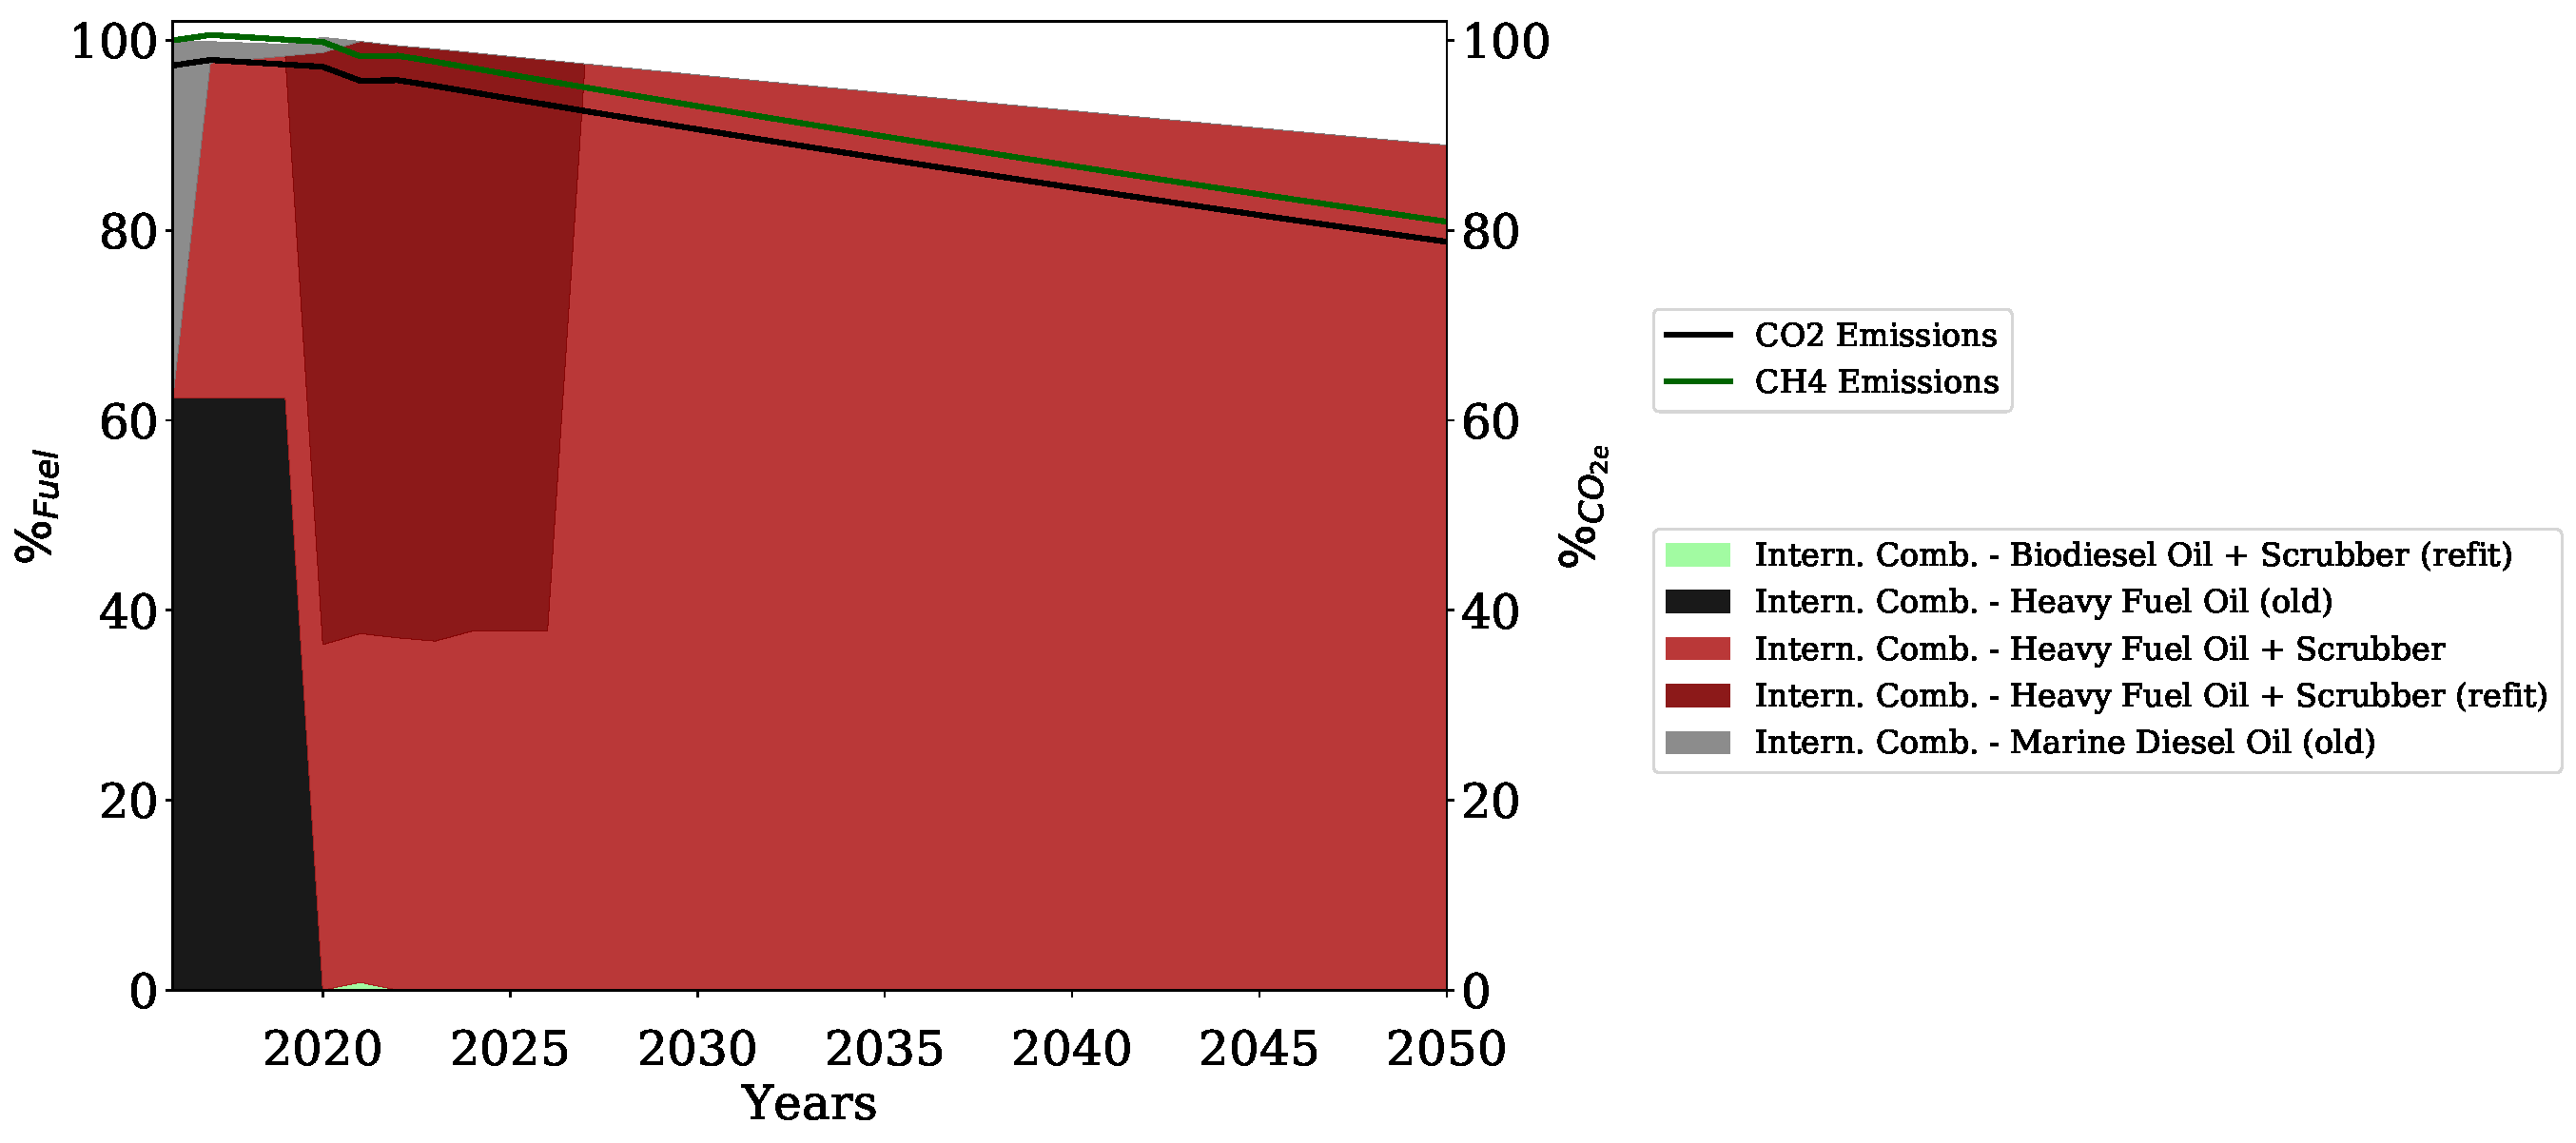
\includegraphics[width=\textwidth]{figures/BAU_fuels_emissions.pdf}
    \caption{Fuel consumption (y-axis left) and cumulative emissions (y-axis right) in the Business-as-usual scenario without carbon budget}
    \label{fig:BAU}
    % TODO: Figure einfügen und am besten auf einer zweiten y-Achse die kumulativen Emissionen reinbringen. Die fuels vll. einfach in % angeben, falls das mit den 16PJ nicht mehr herauszubekommen ist.
\end{figure}

\begin{figure}[htb]
    \centering
    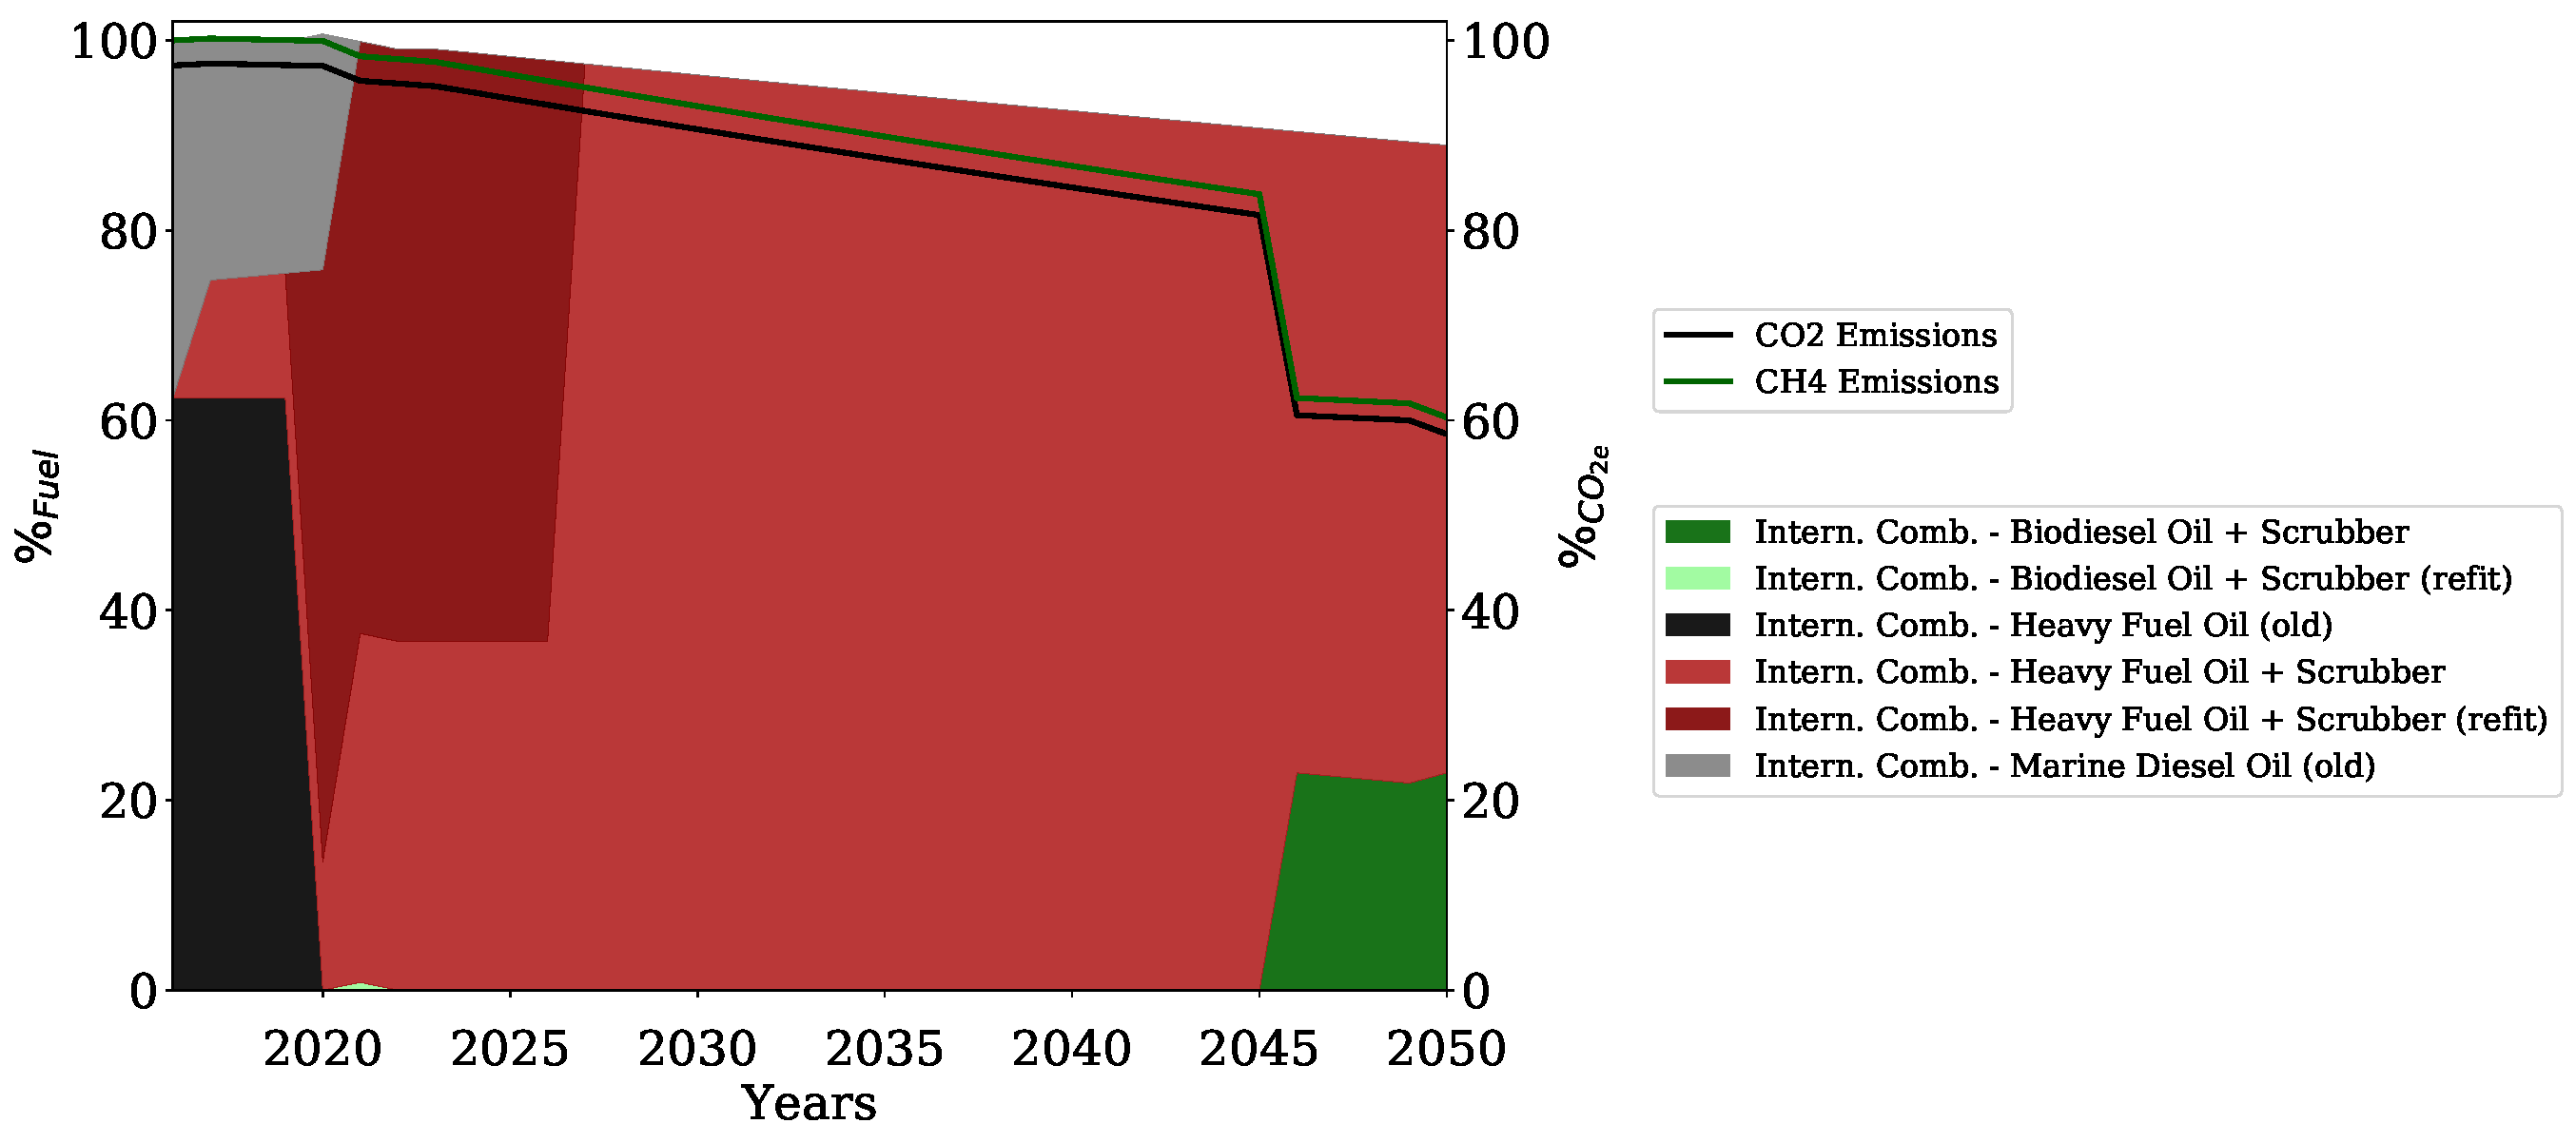
\includegraphics[width=\textwidth]{figures/IMO_fuels_emissions.pdf}
    \caption{Fuel consumption (y-axis left) and cumulative emissions (y-axis right) in the IMO scenario, applying the climate emission target of the International Maritime Organsiation for 2050}
    \label{fig:IMO}
    % TODO: Figure einfügen und am besten auf einer zweiten y-Achse die kumulativen Emissionen reinbringen. Die fuels vll. einfach in % angeben, falls das mit den 16PJ nicht mehr herauszubekommen ist.
\end{figure}

\begin{figure}[htb]
    \centering
    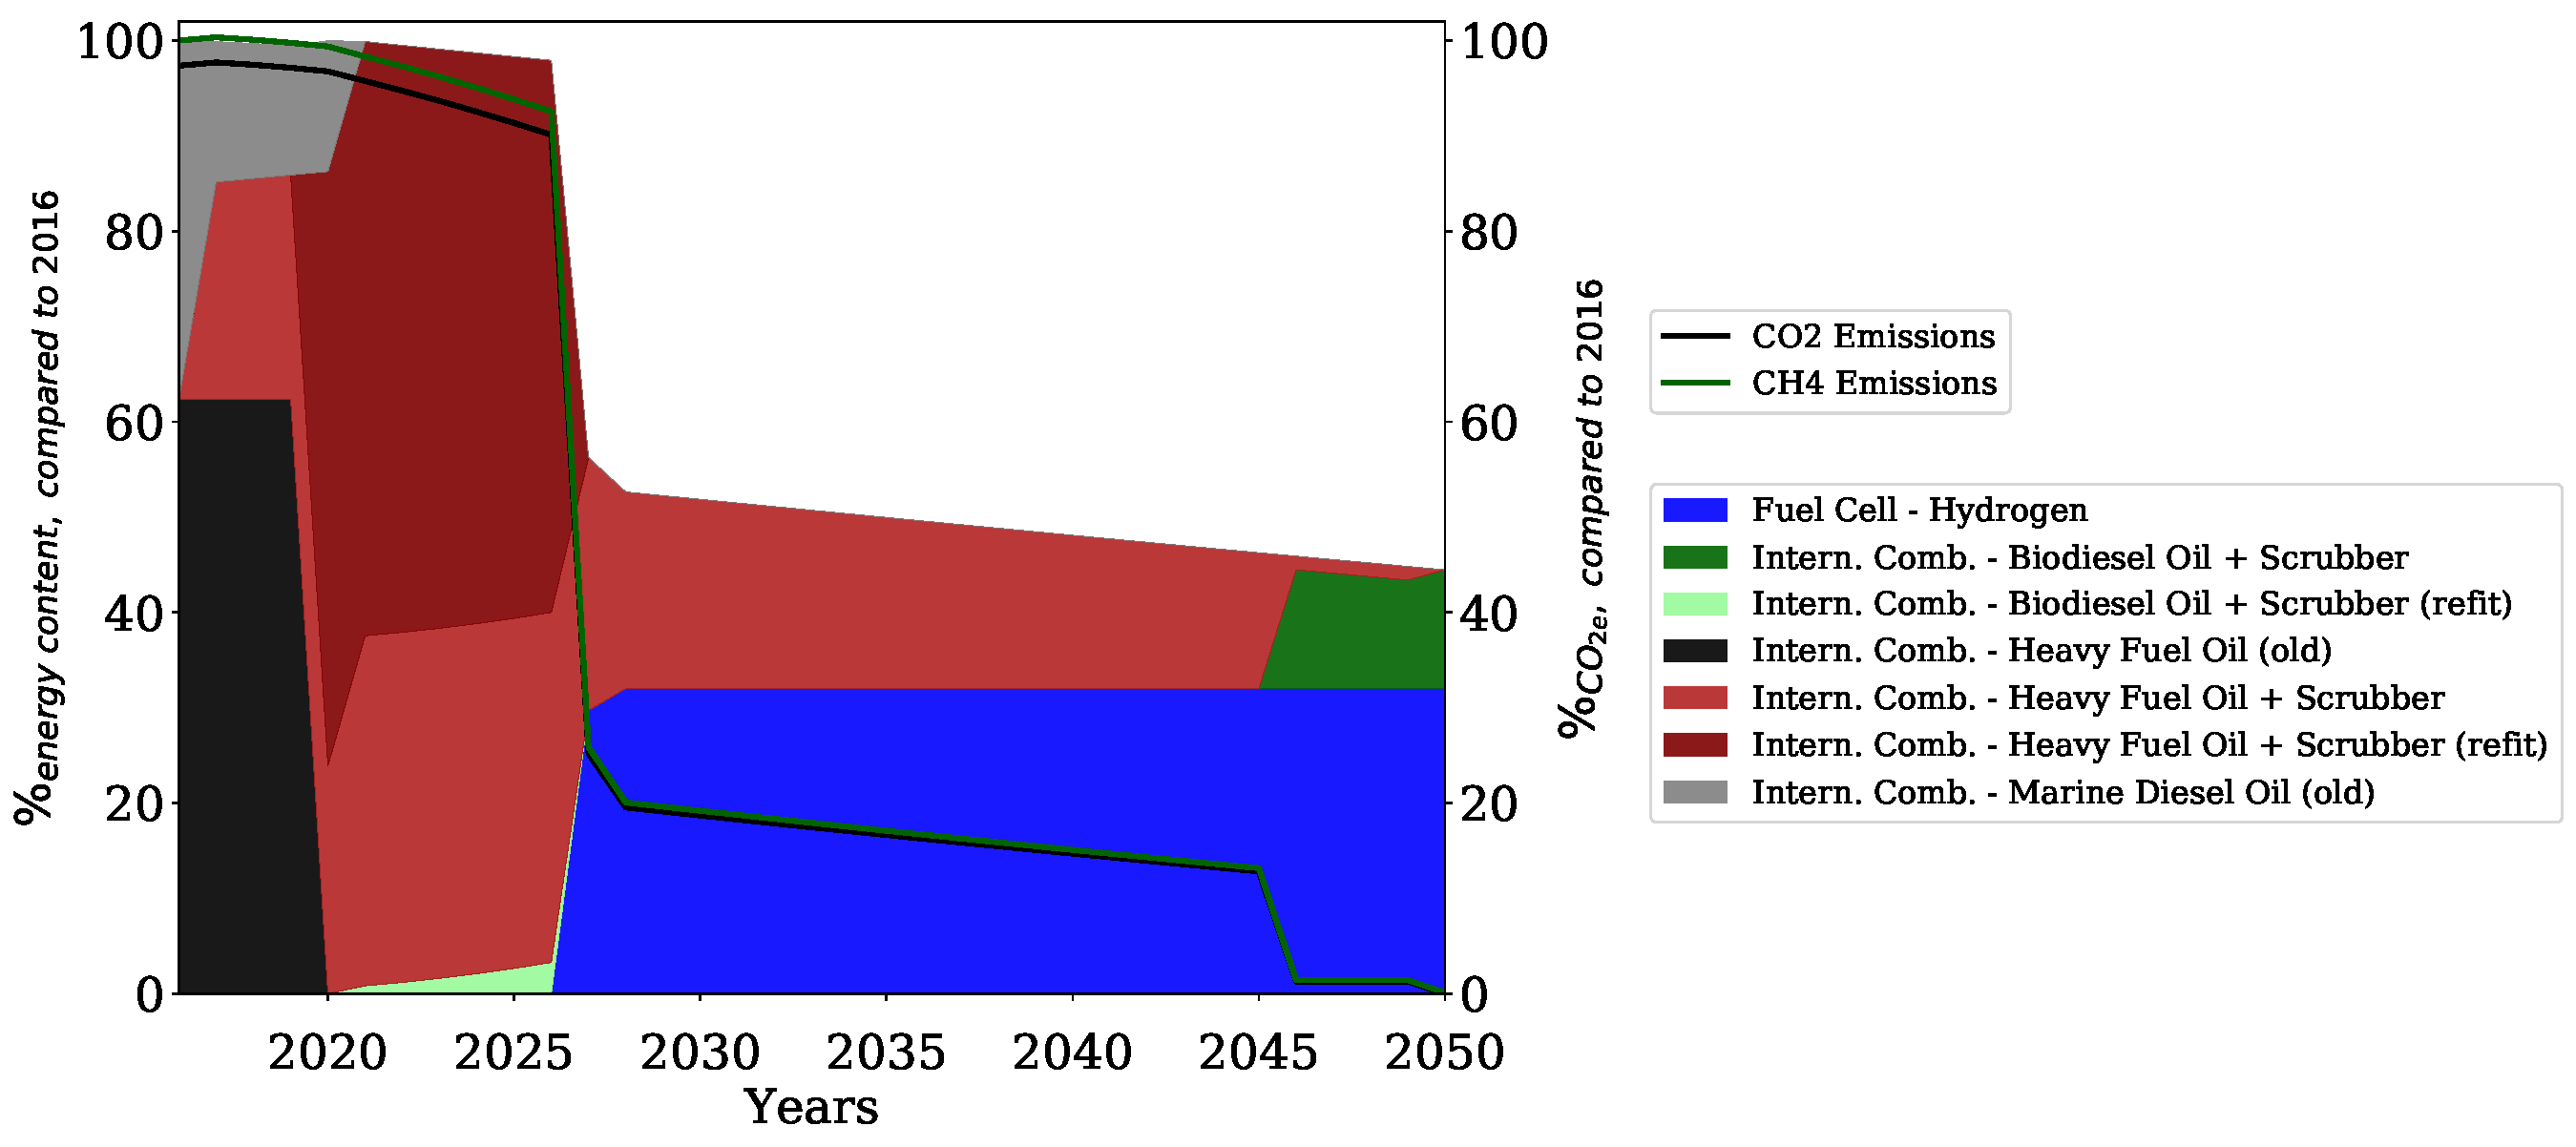
\includegraphics[width=\textwidth]{figures/RS_fuels_emissions.pdf}
    \caption{Fuel consumption (y-axis left) and cumulative emissions (y-axis right) in the Reference scenario with a limited carbon budget}
    \label{fig:REF}
    % TODO: Figure einfügen und am besten auf einer zweiten y-Achse die kumulativen Emissionen reinbringen. Die fuels vll. einfach in % angeben, falls das mit den 16PJ nicht mehr herauszubekommen ist.
\end{figure}

% REF compared to REF methane leakage?
The comparison between the REF scenario with a methane leakage phase out scenario (see \autoref{fig:RS_MP} illustrates the impact, methane emissions have on the possible application of LNG and LBG in a climate emission reduction regime.

\begin{figure}[htb]
    \centering
    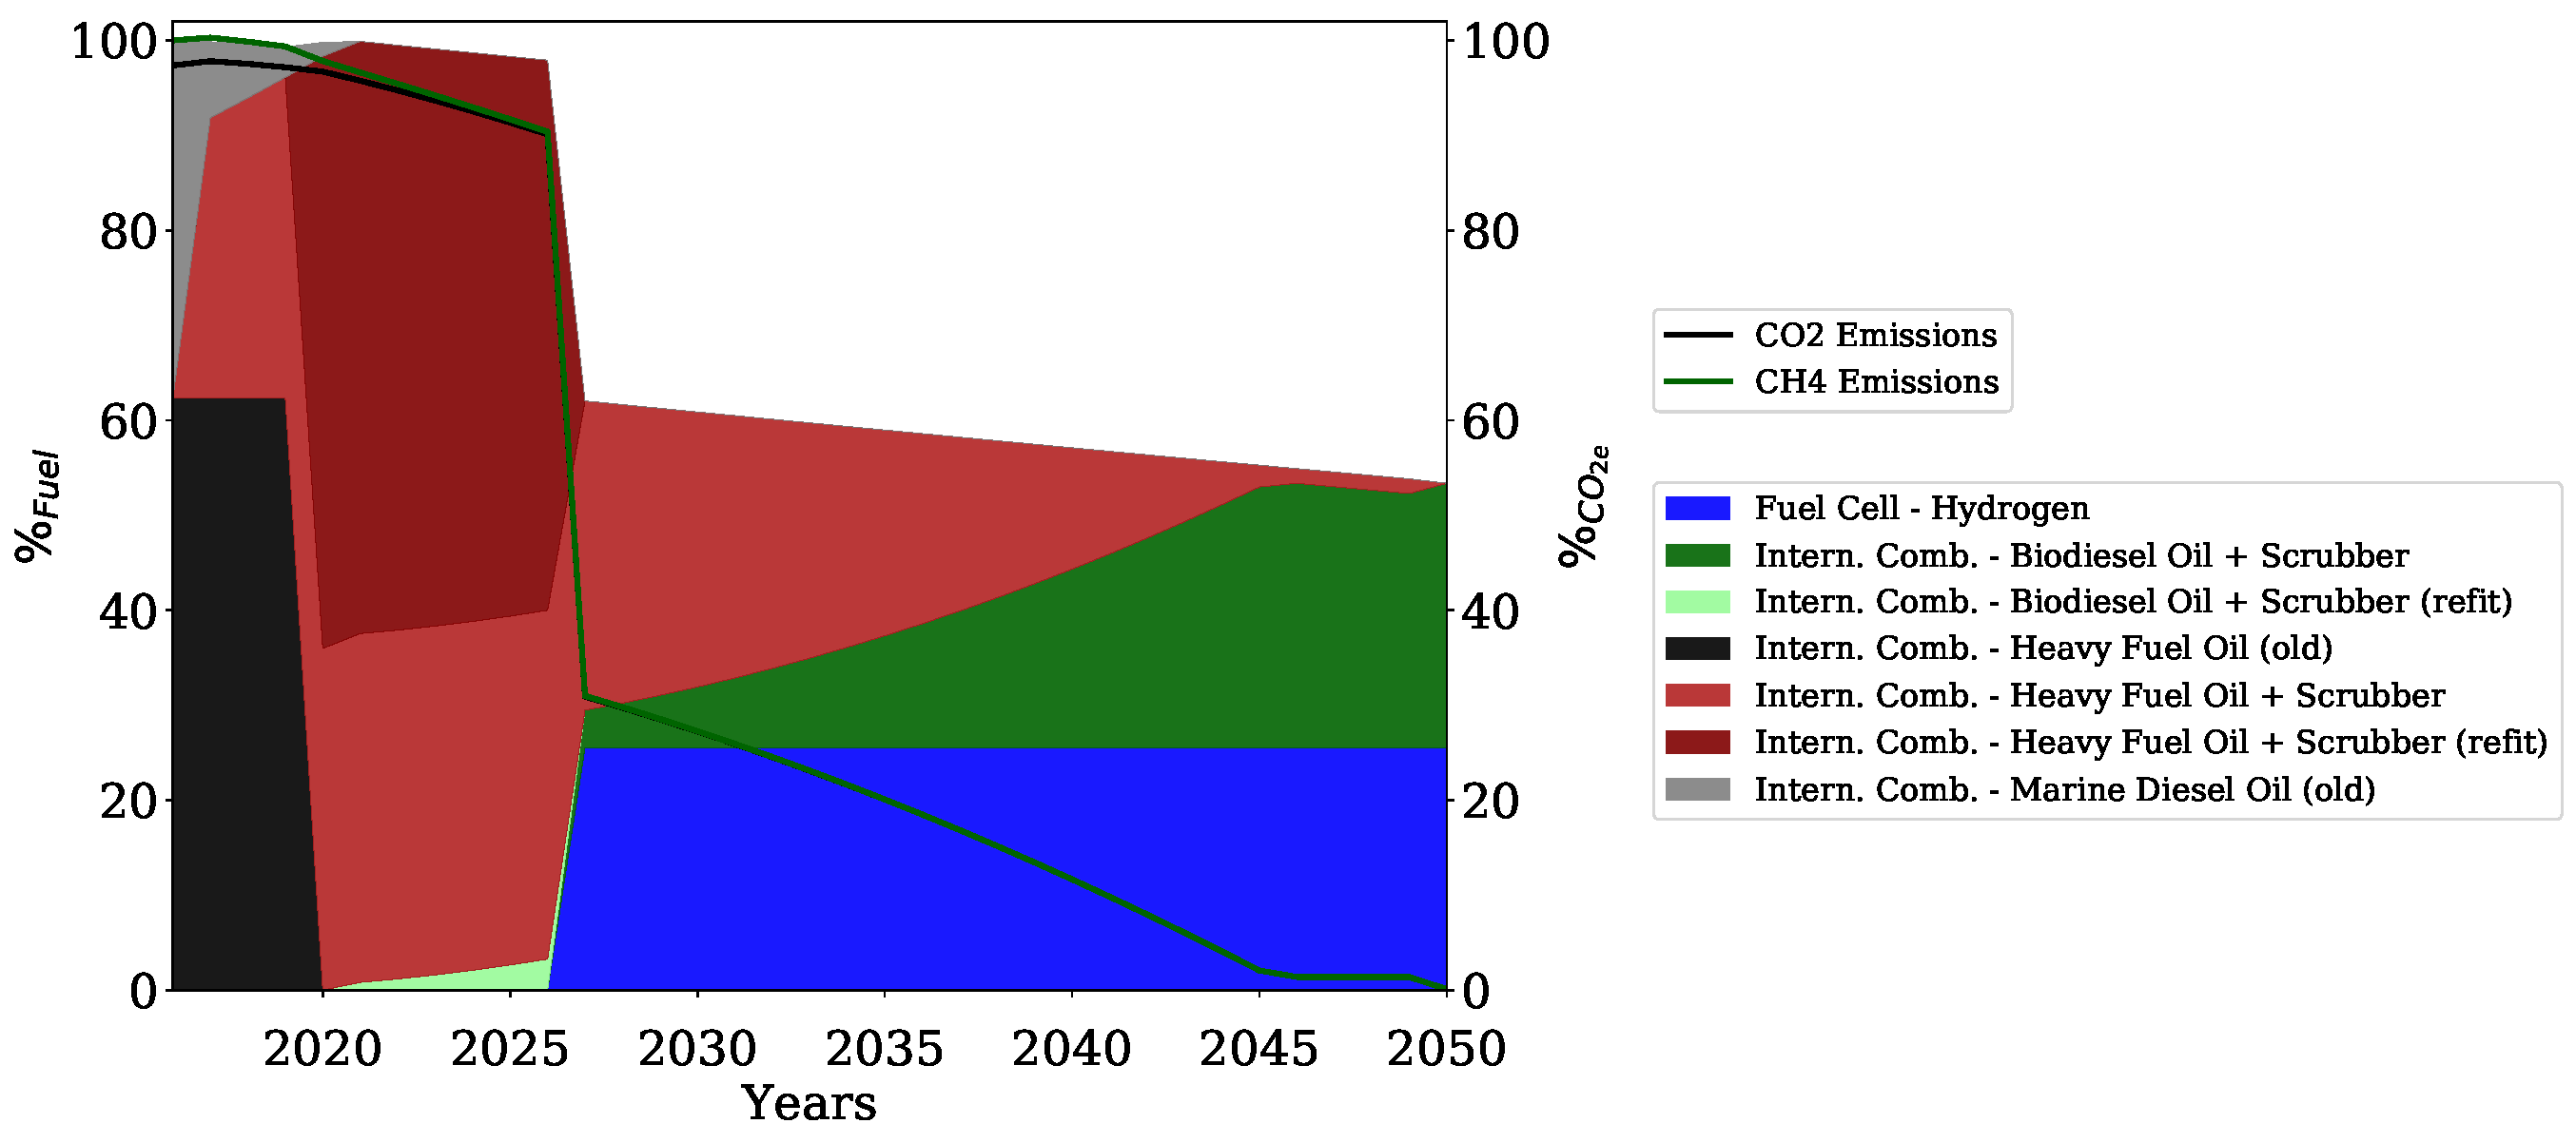
\includegraphics[width=\textwidth]{figures/RS_MP_fuels_emissions.pdf}
    \caption{Fuel consumption (y-axis left) and cumulative emissions (y-axis right) assuming methane leakage phase-out}
    \label{fig:RS_MP}
    % TODO: Figure einfügen und am besten auf einer zweiten y-Achse die kumulativen Emissionen reinbringen. Die fuels vll. einfach in % angeben, falls das mit den 16PJ nicht mehr herauszubekommen ist.
\end{figure}

% Demand variation - Cheapest?, Cost reduction bigger than transport reduction
% aus Tills Arbeit: Since transport demand declines over time, less investments are needed so that the system costs fall by 25 % to 15 billion EUR2016. These overall cost reductions are much greater than the entire transport demand reduction of 17 %. The faster the demand curves in Fig. 8.12 fall before it reaches the year of major investments into new fuel technologies, the greater this cost benefit would be.


% Cost variation: Methanol and Ammonia are close
Due to the high level of uncertainty of cost development of infrastructure, fuel and propulsion technology of different marine fuel options, a wide range of cost variations is applied to test for its effect on fuel composition. The results are summarised in \autoref{fig:costVariation}. Depending on the cost rate change of a specific fuel (x-axis), its share in the total fuel consumption from 2016-2050 (y-axis) changes significantly. The black dashed line at a cost rate change of zero represents the reference scenario. Already at a change of 10\% cost change rate (including fuel, technology and infrastructure costs), methanol and ammonia gain relevance, reaching a dominant role at a 20\% cost change rate.

% LNG is no option, LBG just if methane leakage phase out
For LBG, the development of the methane leakage problem is of outstanding importance. Under the assumption that methane leakage can be coped with until 2050 (dashed line), LBG is close to hydrogen, methanol and ammonia as choice to be the dominate fuel in 2050. Contrary to that, LNG would not only require a methane leakage phase out, but also a very favourable cost development to play a major role.

% BATW has to be decreased significantly, but the conditions applied were rather unfavorable for BATW.
Sailing cargo ships, driven by a combination of wind and electricity from batteries seem to only be cost efficient in case of very strong drops in costs. However, the influence factors have more dimensions than just the pure battery and ship costs. In this model, it is assumed that one third of the propulsion is done by electricity. For long distance cargo, that mainly has to use the engine for manoeuvring into and out of the harbour, the wind share and potentially additional solar input can be significantly increased and thus the required battery and electricity costs reduced.

\begin{figure}[htb]
    \centering
    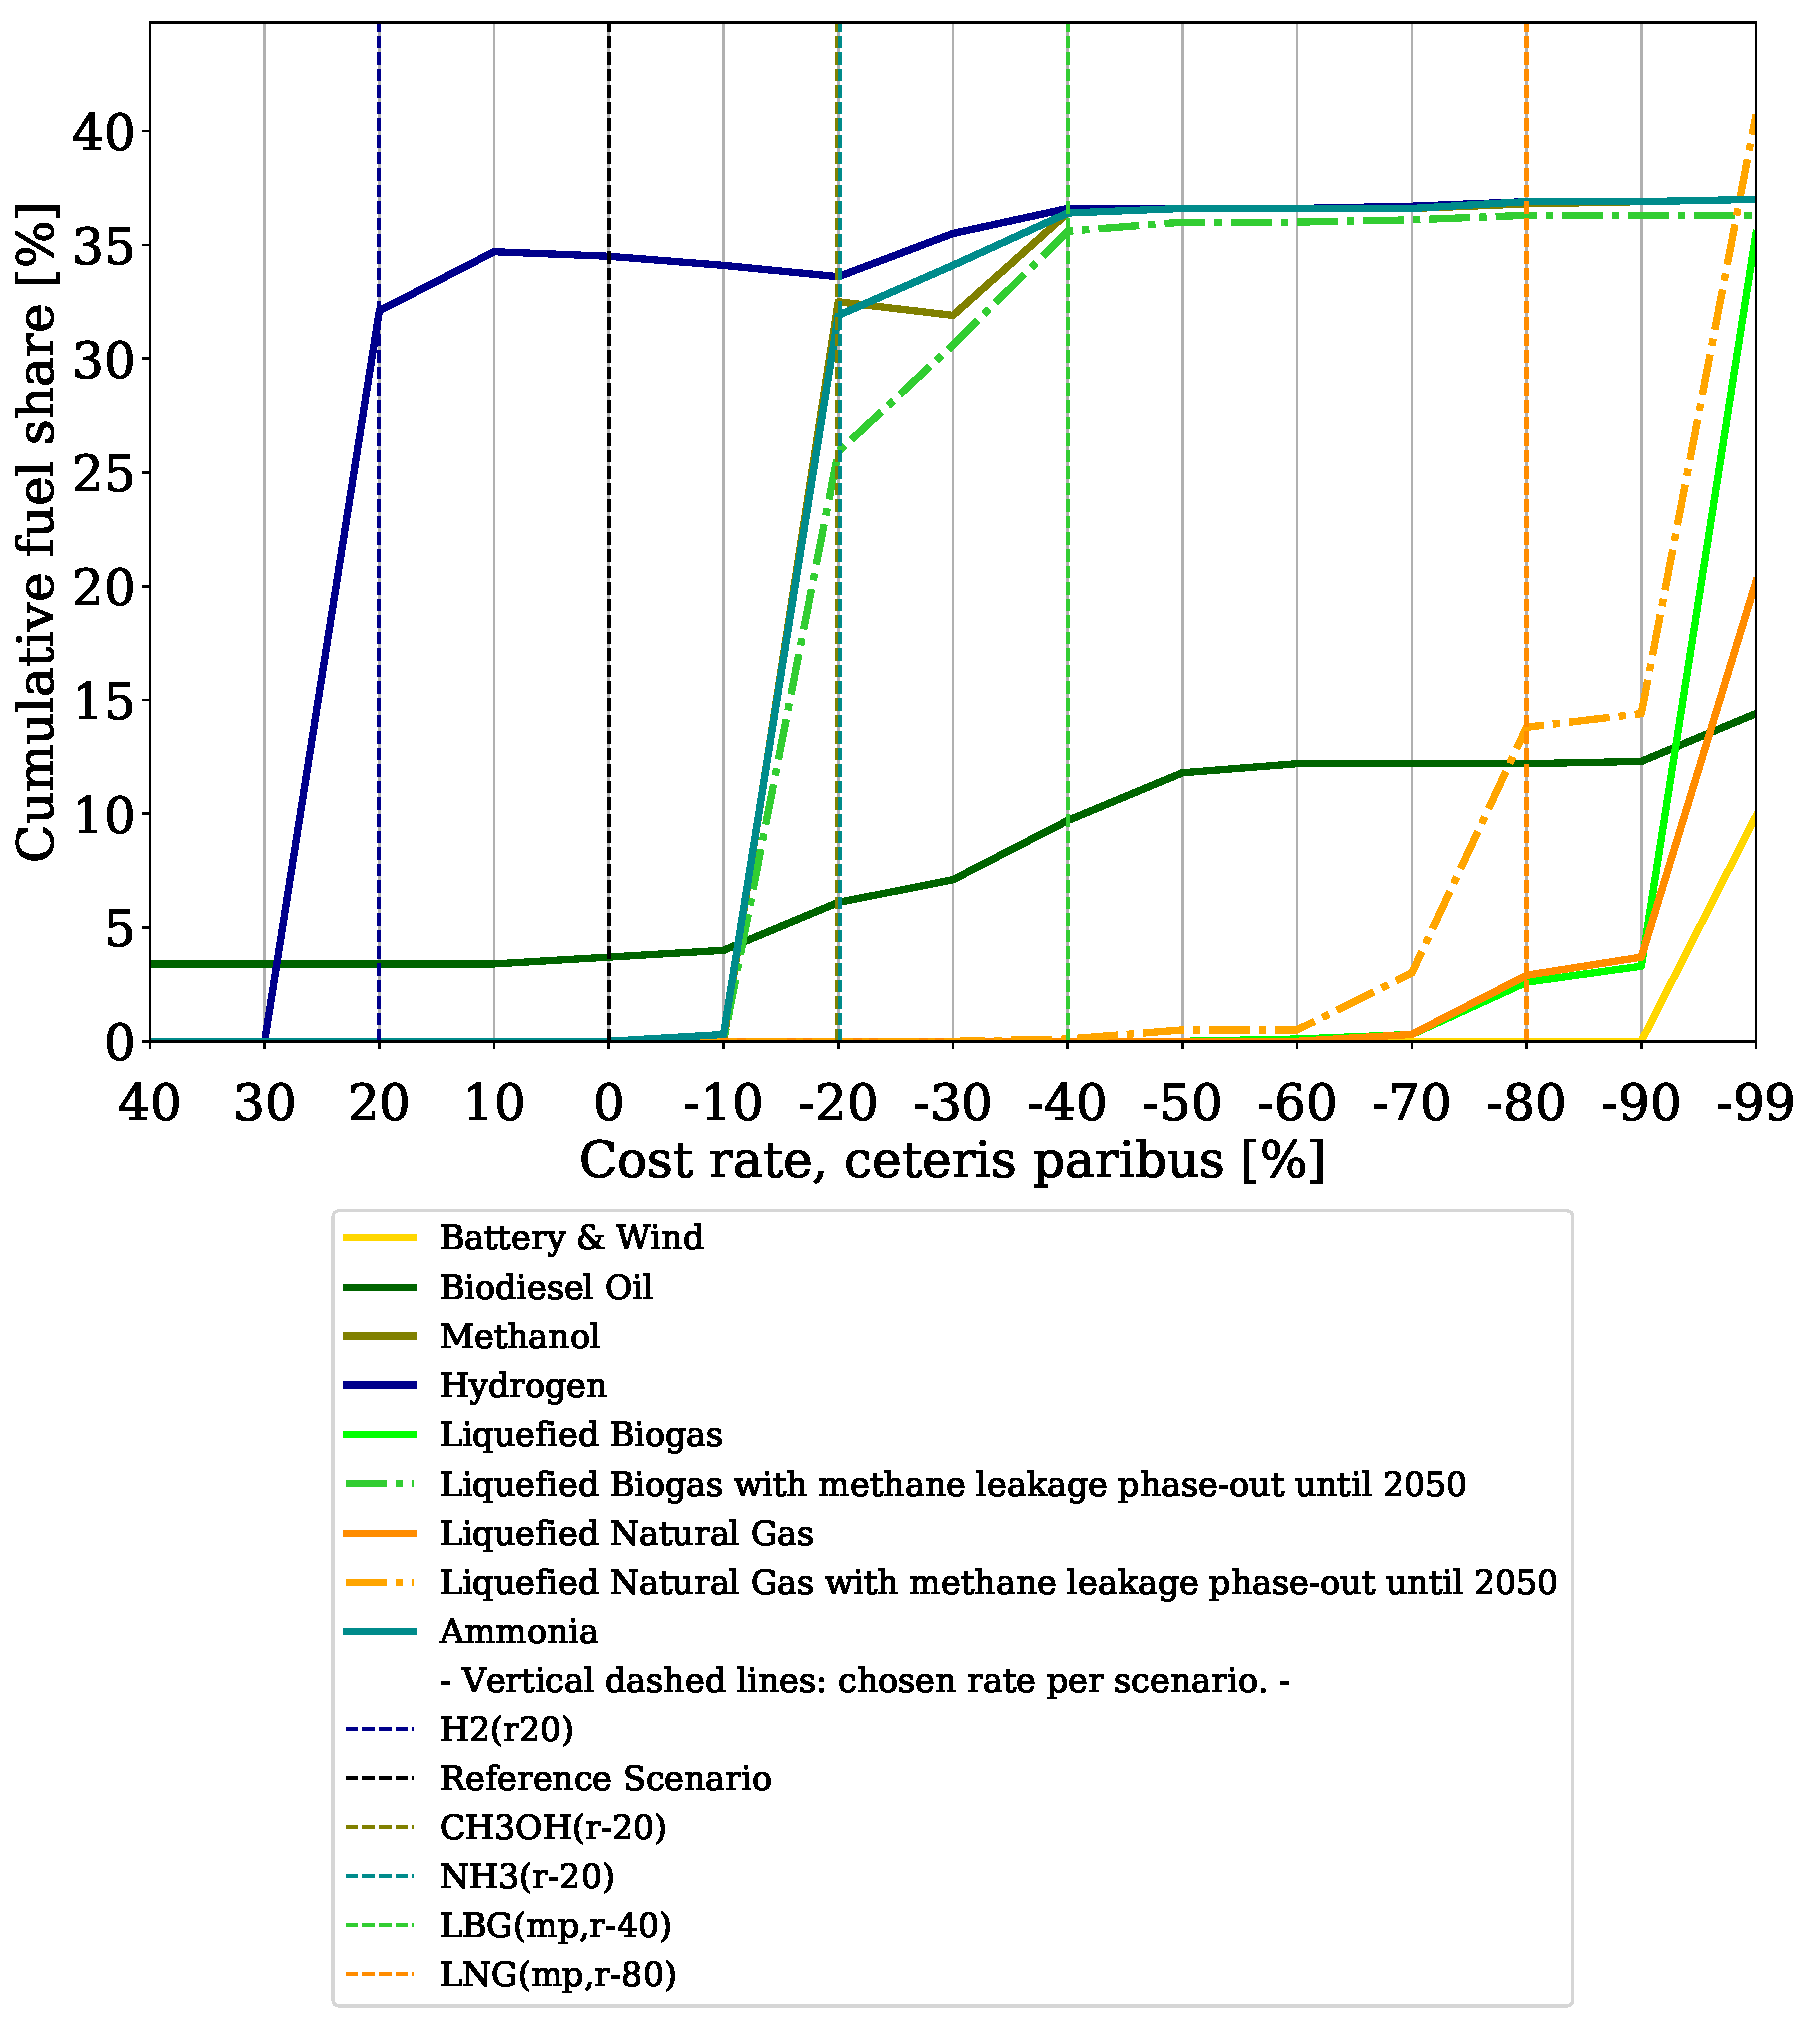
\includegraphics[width=\textwidth]{figures/costVariation.pdf}
    \caption{Total fuel shares from 2016-2050 (y-axis) in relation to different cost range changes (x-axis) compared to the reference case}
    \label{fig:costVariation}
    % TODO: Figure einfügen mit ausfuehrlicheren Fuel Namen
\end{figure}

% Compare all scenarios: Fuel composition total and 2050
For comparison, the total fuel use of all scenarios for 2016-2050 is displayed in \autoref{fig:AllFuelTotal} and the fuel composition in the target year 2050 in \autoref{fig:AllFuel2050}. A general efficiency increase can be seen for all carbon budget scenarios. Due to higher efficiencies and thus a higher Tkm/GJfuel - rate, less fuel is applied in the carbon budget scenarios. Except the transport demand scenario all supply the same transport demand.

\begin{figure}[htb]
    \centering
    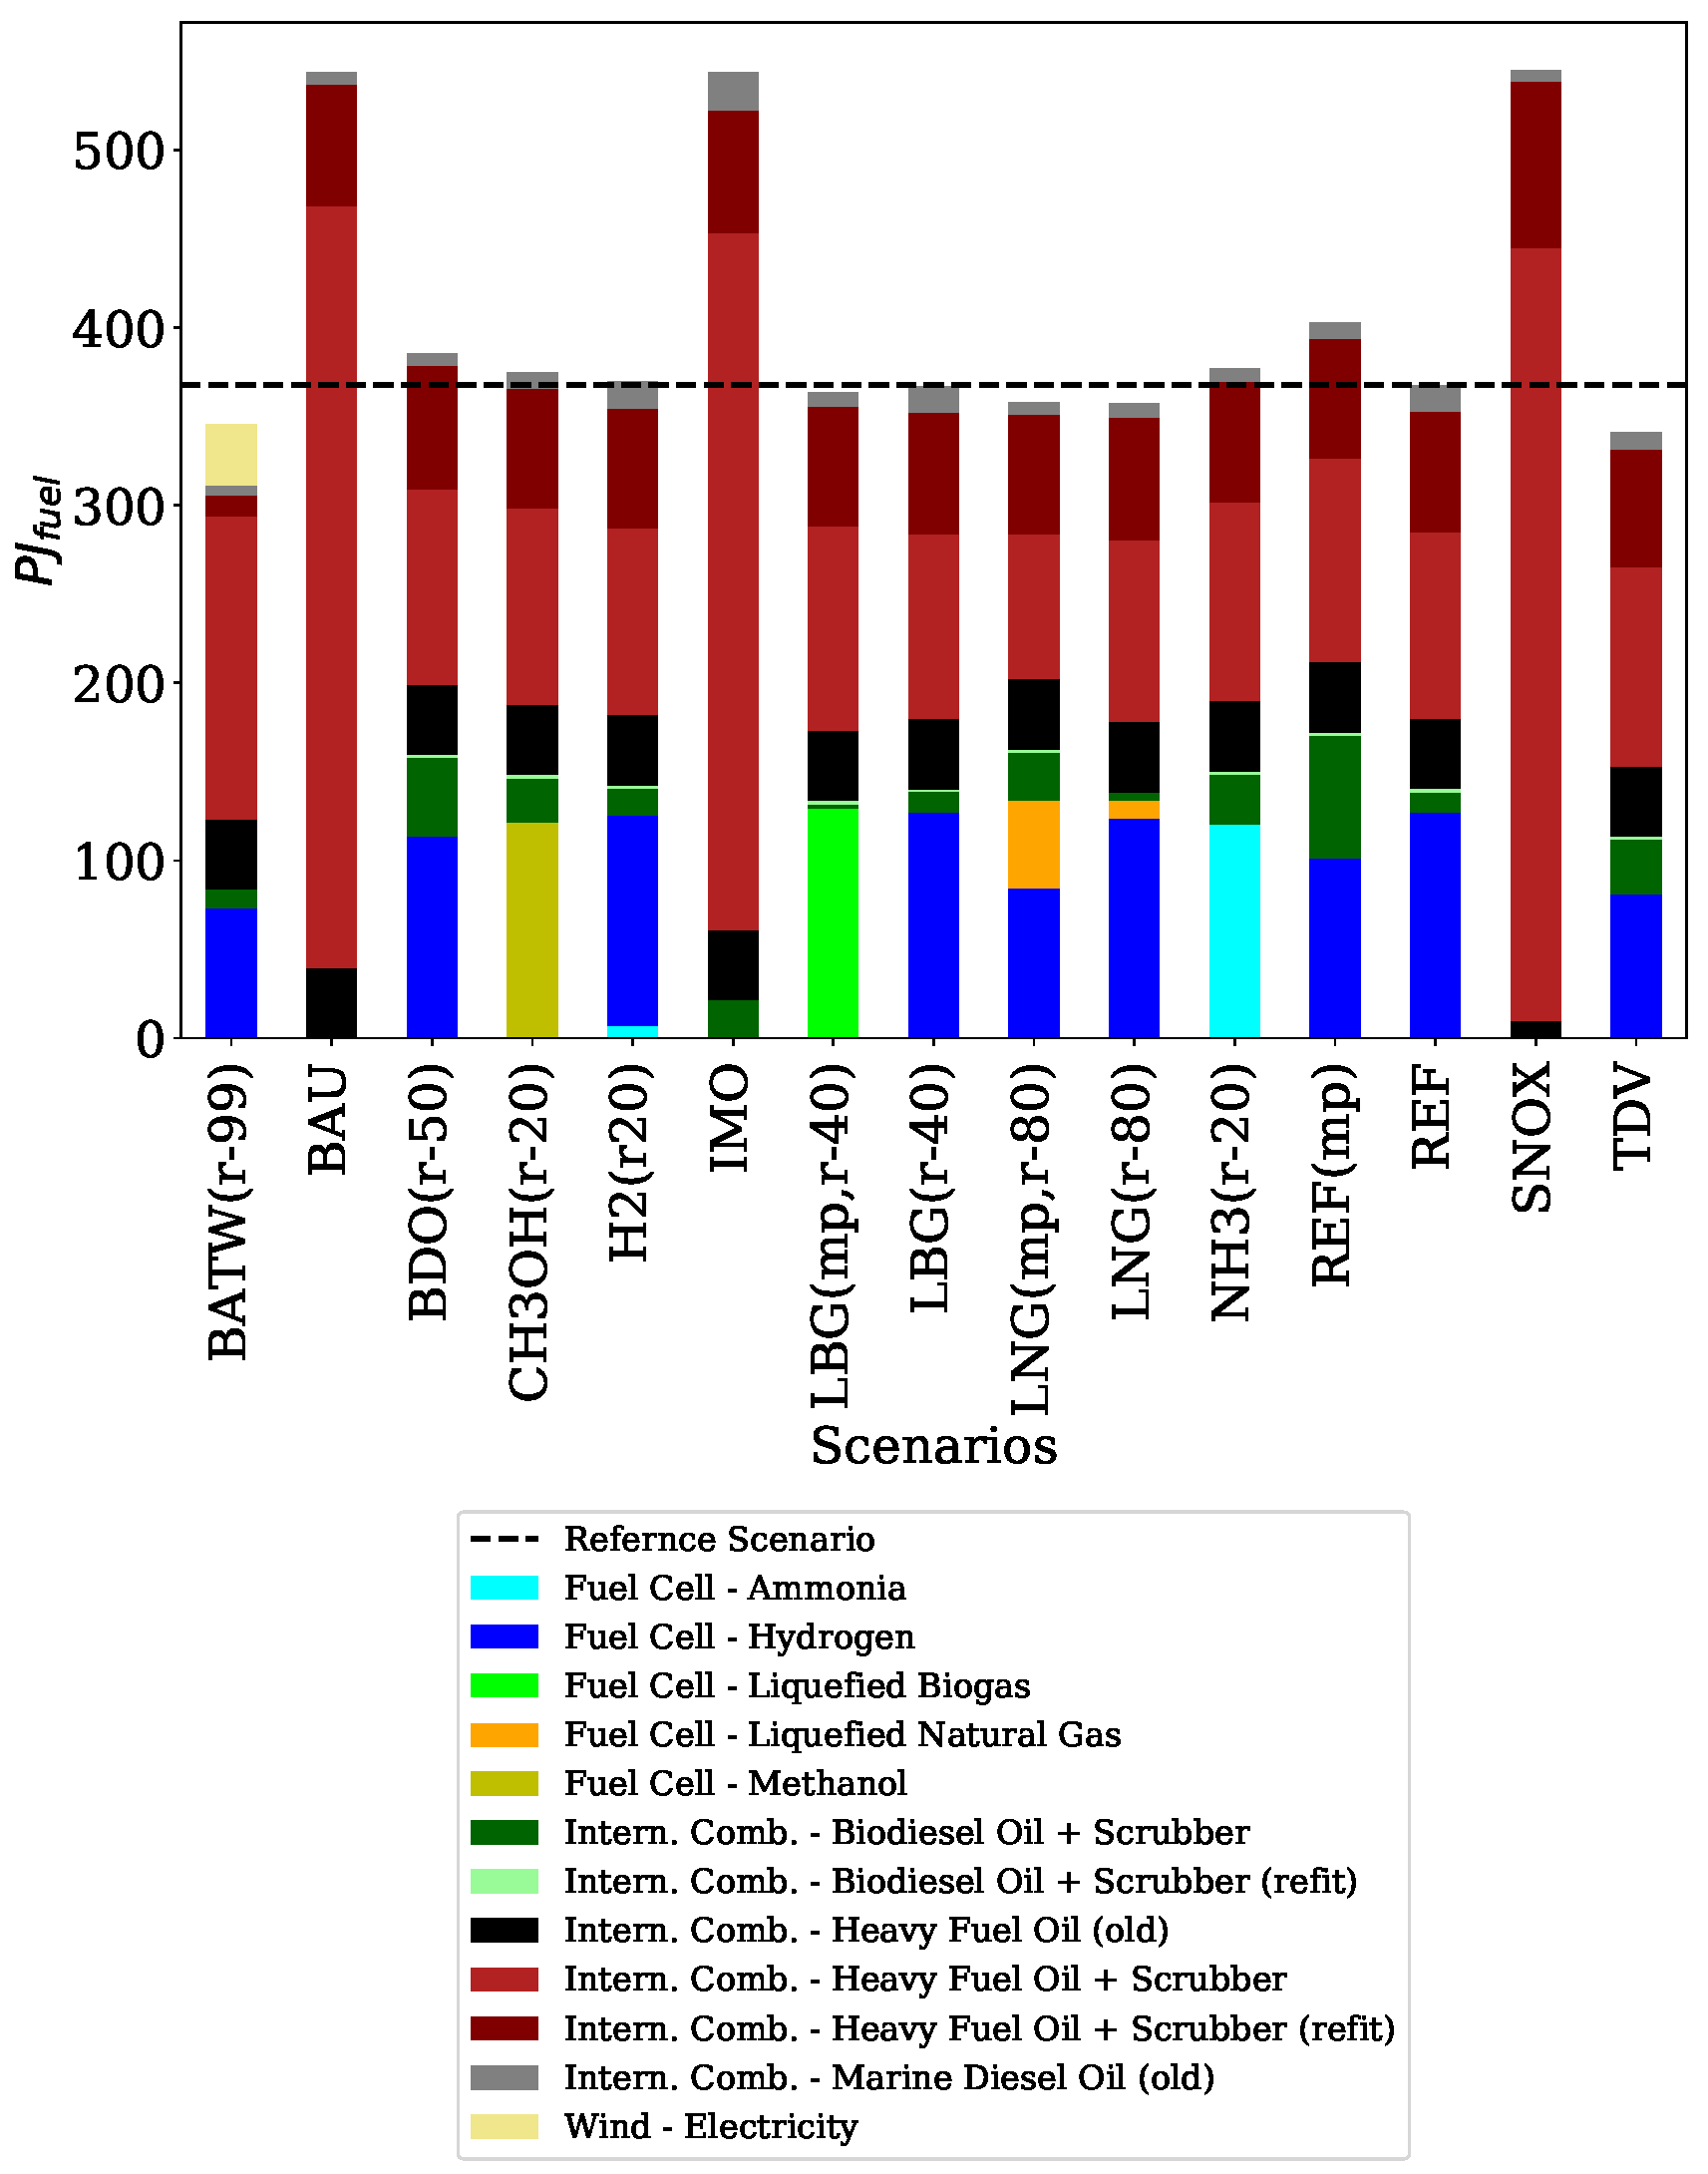
\includegraphics[width=\textwidth]{figures/AllFuelTotal.pdf}
    \caption{Total fuel use from 2016-2050 for all scenarios}
    \label{fig:AllFuelTotal}
    % TODO: Figure einfügen mit ausfuehrlicheren Fuel Namen
\end{figure}

\begin{figure}[htb]
    \centering
    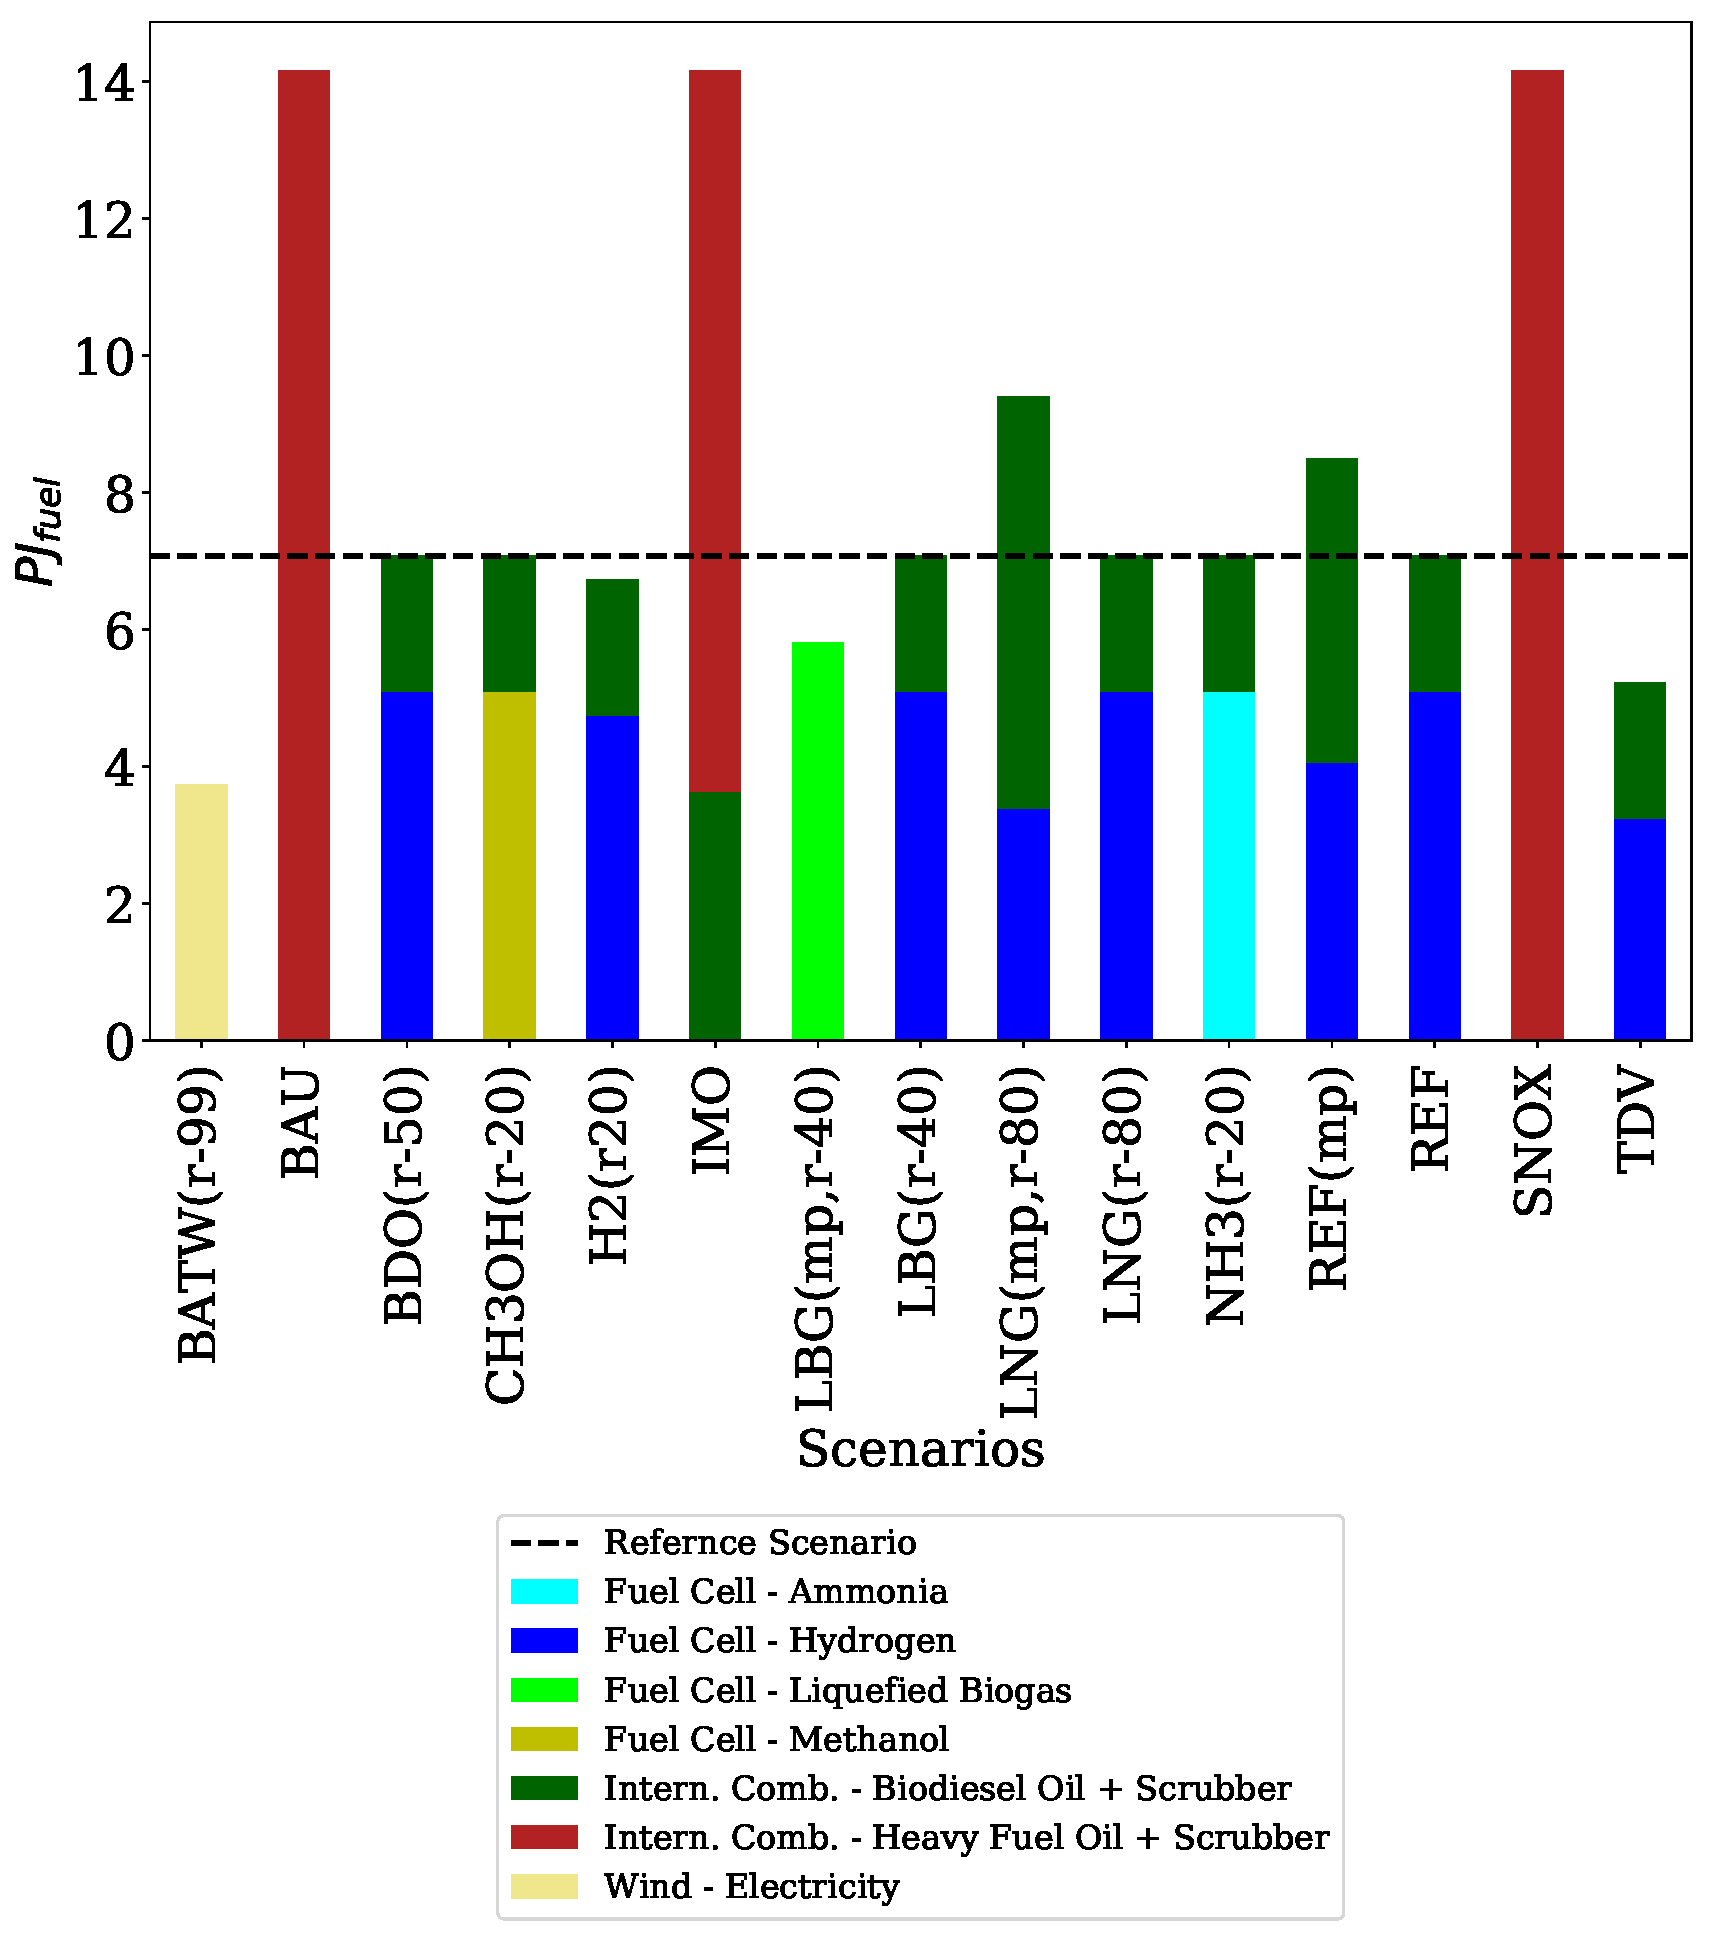
\includegraphics[width=\textwidth]{figures/AllFuel2050.pdf}
    \caption{Fuel composition in 2050 for all scenarios}
    \label{fig:AllFuel2050}
    % TODO: Figure einfügen (die hab ich bisher noch nicht gesehen, hoffe die ist nicht kompliziert zu machen?) EVENTUELL BEIDE GRAFIKEN NEBENEINANDER UND DAMIT IN EINE PACKEN
\end{figure}

% Compare all scenarios: Costs - not sure if there should be a figure - maybe rather include the full table of results

% Costs - resulting EURO/CO$_2$e
Derived from the cost differences for fuel, ship and infrastructure, a carbon price in the range of 350--450 \euro(2016)/ton CO$_2$e would be required for a renewable transition of the Danish shipping sector. [Rau17, p. 198] TODO:insert citation - reports similar prices of around 430 \euro(2013)/ton CO$_2$e for a global transition.

% applicability of the model on other countries
% applicability of the findings for the world shipping
The model code and most of the data references and preprocessing can also be applied for other countries, especially Europe. However, since shipping has a global perspective, the case study for Denmark already gives a good indication of the fuel shares chosen for a cost-optimal path to carbon neutrality in 2050 for the worldwide shipping. Conditions for shipping are similar, the basic parameters, technology, fuel and infrastructure costs are considered as world prices rather than reflecting local particularities. This is also reflected and validated by the similar CO$_2$e-cost range compared to other, worldwide studies. 

% Why the mentioned costs are rather the upper end
Compared to other sectors like electricity and heat, these mitigation costs per /ton CO$_2$e seem high, one has to consider several points. First, this is the upper bound of cost: Technologies considered are all applicable today, developments in other sectors applying similar fuel switch options could further increase costs, additional alternatives could evolve. Second, as shown in the demand reduction scenarios, any decrease in transport demand would save costs even beyond the proportional saving. And third, refits and hybrid solutions have not been considered to a great extent in the model functionality and could further decrease costs and ease the shift to different fuels.

% Costs - what does that mean for the cargo cost

% Co-benefits.
Thus, costs could get lower for the transition, but the question is also whether to talk about mitigation costs. Co-benefits like reduced air pollution have not been quantified on a monetary basis in the model and were this not part of the optimisation. However, these could have essential health benefits, maybe even reaching mitigation gains instead of mitigation costs.

% Regulation / Recommendations
The necessary transition will not happen under current market conditions. Regulation is required urgently to bring shipping on the pathway to carbon neutrality in 2050, in line with the Paris Agreement. A carbon budget for shipping worldwide, broken down to countries is a viable option to consider. Additionally research money for alternative fuels and technologies, as well as solving crucial questions on security, infrastructure and methane leakage issues are important contributions to implement the transition to climate neutral shipping in 2050. 

% might be missing: strengths ad weaknesses of te model.

\section{Conclusion}
% 250 words
% only draft until now!
The achievement of CO$_2$-neutrality in the shipping sector is of great importance for reaching the targets of the Paris Agreement. Although this goal is underrepresented in the current discussion, this study shows, that it is possible for the Danish part of international shipping to become CO$_2$-neutral until 2050 with existing technologies. Regarding fuels, hydrogen, methanol and ammonia are from a socio-economic cost perspective the most compatible. Due to high uncertainties regarding future cost developments and safety requirements (esp. ammonia), there is no clear winner. Regarding technologies, fuel cells are chosen for these fuel options, the decisive parameter being the higher fuel efficiency. Although LNG is the fuel option most prominently discussed as an alternative today, it would only have a short window of opportunity, mainly because of leakage problems of methane causing high greenhouse gas emissions as well as high fuel and technology costs. If this gaseous fuel is based on renewable sources, the so-called LBG can only play a role if methane leakage can be drastically reduced until 2050. The option of cargo-ships driven by a mixture of wind and electricity stored in batteries could not adequately be represented in the model setting. The evaluation of their role would need a further refinement of the calculations.
%Although additional conditions for the future application of fuel for shipping like safety issues or infrastructure decisions are not reflected in the model, ...
The presented modelling approach indicates that either strong regulative carbon budgets or a carbon price of 350--450 \euro/t~CO$_2$e would be required to induce the necessary changes for a carbon neutral Danish shipping in 2050. This would double today's average cargo transport costs. However, due to the low share of transport cost on the value of transported goods, the average transported good would only increase by 6\% on average. This can be considered as the upper limit, since new fuel possibilities not reflected in this study might evolve.

\section*{References}

\bibliography{mybibfile}

\end{document}